\section{IoT}
Sempre più spesso si parla di Internet delle cose, o IOT, con questo termine si 
intende un evoluzione delle applicazioni legate al settore mobile, al settore
della home automation e al settore embedded. 
In questo scenario ogni oggetto il
quale contiene un sensore sarà connesso ad Internet. Avvalendosi di questa
connessione , i vari dati raccolti potranno essere inviati nel cloud, dove
verranno elaborati e resi disponibili alle varie applicazioni. 
Per fare in modo che questo update avvenga, è necessario riuscire a creare una
rete di devices ,correlati nelle loro funzionalità, i quali riescano a
\emph{parlare un linguaggio comune}. \improvement{Scrivi qualcosa di decente
qui}
Il punto principale di questo
upgrade sta nel riuscire a creare una rete di devices connessi ad internet. Per
supportare e utilizzare una potenza di calcolo maggiore andando a combinare
tecniche di data analytics per estrarre le informazioni più significative. 

In
questa visione, milioni di devices saranno connessi a Internet e molto presto
milioni di milioni di devices. 

Il mercato di questi \emph{smart devices } è
in rapida crescita con una stima di 8,3 miliardi di dispositivi connessi nel
anno 2017, e di circa 20 miliardi per l'anno 2020 \cite{gartner2016}. Andando ad
creare un impatto economico compreso tra i 2.7 e i 14 trilioni di dollari. I
mercati principali saranno quelli del healt care con un introito compreso tra i
$1.1$ e i $2.5$ trilioni di dollari e il settore industriale con $2.3$ a $11.6$
trilioni di dollari.

\begin{figure}[h]
\centering 
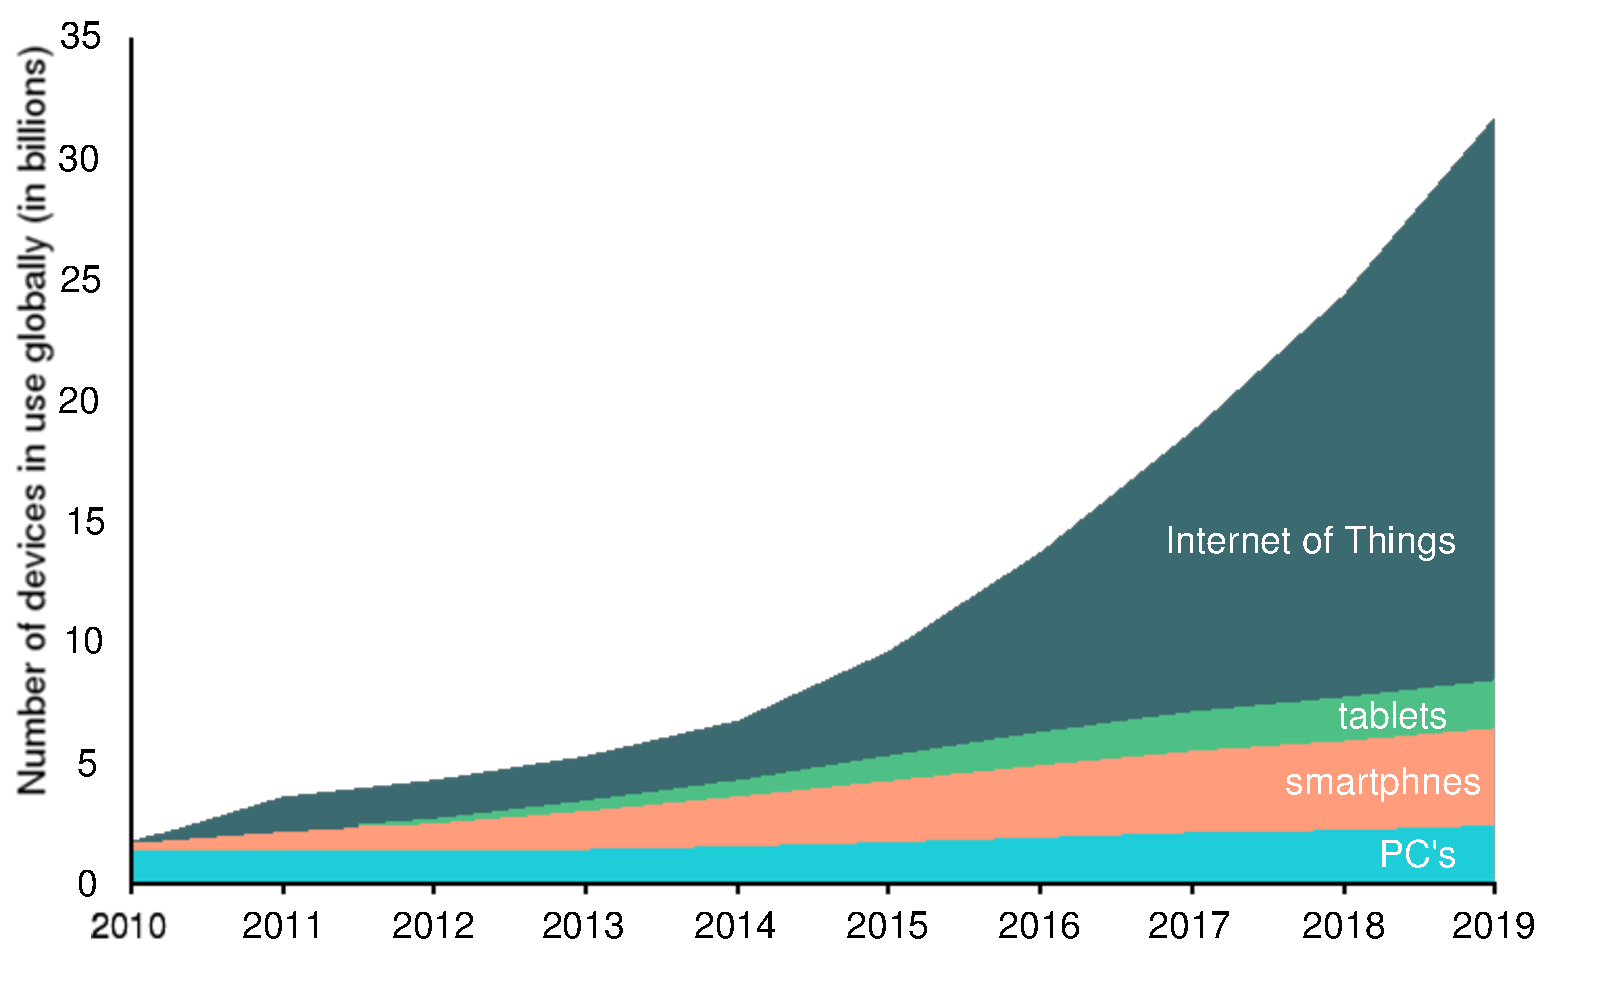
\includegraphics[width=10cm]{iot_devices}
\caption{Numero di dispositivi per anno}
\end{figure}

Questa rapida crescita ha portato alla ricerca è sviluppo di nuove soluzioni 
tecnologiche per supportare il carico di dispositivi simultaneamente connessi 
alla rete, senza avere un degrado evidente delle performance.
Per non alterare il \emph{QoS} Quality of Service della rete , hardware e
software dovranno essere rivisti insieme alla topologia di rete utilizzata. I
principali punti chiave sono

\begin{itemize}
\item \textbf{Scalabilità}: Dato l'elevato numero di devices connessi, scenari
urbani ed industriali, la network tecnologi alla base dovrà essere estremamente
adattabile, in maniera dinamica, al carico di dispositivi connessi.
\item \textbf{Costo unitario}: Il costo del singolo modulo, dovrà essere basso
per garantire la più ampia fetta di mercato.
\item \textbf{Durata della batteria}: La maggior parte dei dispositivi sarà
alimentata tramite batteria, e la durata media e stimata di anni. 
\item \textbf{Costo computazionale}: La modulazione alla base di queste nuove
tipologie di rete, dovrà essere concepita in modo da non avere un costo
computazionale elevato.
\item \textbf{Distanza}: Un altro punto fondamentale è la possibilità di avere
comunicazioni a lunga distanza.
\item \textbf{Sicurezza}: Ogni devices dovrà essere difficilmente penetrabile da
attacchi esterni.
\item \textbf{Menagment}: I vari dispositivi dovranno essere facilmente
controllabili da remoto.
\item \textbf{Fail-safe}: Il non funzionamento di devices non dovrà
compromettere l'intera infrastruttura a lui connessa. 
\end{itemize}

Vari tipi di architetture di rete sono stati proposti per realizzare questa
nuova infrastruttura. Per quanto le varie proposte si basano su tecnologie
differenti, è possibile individuare tre layer comuni 
\begin{itemize}
\item \textbf{Device layer} formato da tutti i dispositivi che collezionano dati
e sono connessi alla rete.
\item \textbf{Network layer} La struttura della rete, la quale permette di
connettere i vari devices in modo che possano scambiare i dati tra di loro o
inviarli ad un data-center.
\item \textbf{Application layer} il quale interpreta e utilizza i dati ricevuti.
\end{itemize}

Questo comporta delle sfide sia dal lato hardware sia dal lato software. 
Infatti
questi devices dovranno essere economici , avere una lunga durata della batterie
dal punto di vista hardware. Dal punto di vista software, dovranno essere sicuri
e dovranno essere facilmente controllabili e lavorare in maniera semi autonoma.
Oltre a ciò la  sfida è riuscire a creare delle sottoreti di devices relazionati tra di loro
riuscendo a creare un linguaggio comune per lo scambio delle informazioni ,
realizzando un sistema autonomo ed intelligente di sistemi intelligenti. Il
tutto si basa sull'utilizzo del cloud e l'analisi dei dati per far in modo di
migliorare la maggior parte dei settori, quali buisness, healt care, il
settore manifatturiero e quello delle energia per fare alcuni esempi, producendo
in maniera più veloce e con costi ridotti. 

cos'è una cosa , una cosa è qualsiasi tipo di oggetto il quale ha un sensore e
invia dati nel cloud in modo tale che quei dati possano essere analizzati e
riutilizzati , internet cellulari , tutto questo hanno cambiato il modo in cui
facciamo le cose, sia in modo personale sia nel mondo del bisnes  cosi anche
l'internet delle cose cambierà il nostro modo di fare le cose . Ci sono delle
sfide riguardo i devices che sono sia hardware che software come il consumo
della batteria e menagment, il fatto di non venire interrotti e compatibilità,
poi ci sono le sfide per creare sistemi che riescano a processare tutti i dati
genereati e riuscire a fare delle azioni intelligenti , problemi riguardo alla
sicurezza e privacy più ci muoviamo verso un modo sempre più connesso queste
difficolta diventano sempre più predominanti e difficili da risolvere

punti principali per i devices
\begin{itemize}
\item connettività
\item sicurezza
\item controllo
\end{itemize}
